\chapter{Lernverfahren}
\section{Entscheidungsbäume}
Entscheidungsbäume dienen der Klassifizierung von Daten.
Die Inneren Knoten sind dabei die Attribute und die Blätter stellen die Zielvariablen da.
\begin{figure}[htbp]
	\centering
	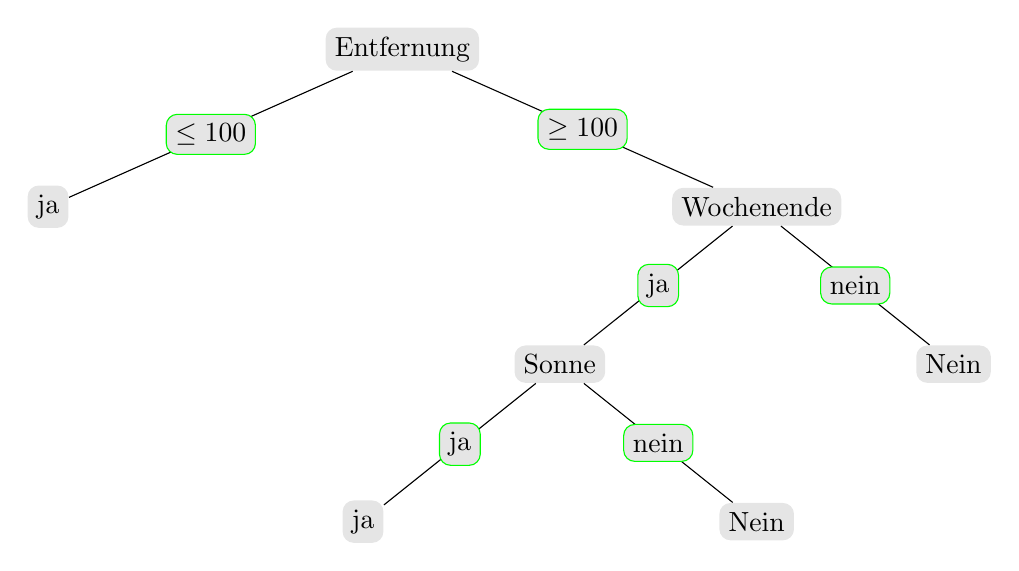
\begin{tikzpicture}
		[every node/.style={fill=black!10,rounded corners,align=center},
		grow=south, level distance=2cm,
		level 1/.style={sibling distance=9cm},
		level 2/.style={sibling distance=5cm},
		]

		\node{Entfernung}
			child{
				node{ja} edge from parent node[draw=green]{\(\leq 100\)}}
			child{
				node{Wochenende}
					child{
						node {Sonne}
							child{
								node {ja}edge from parent node[draw=green]{ja}}
							child{
								node {Nein} edge from parent node[draw=green]{nein}}
						edge from parent node[draw=green]{ja}}
					child{
						node {Nein} edge from parent node[draw=green]{nein}}
					edge from parent node[draw=green]{\(\geq 100\)}}
		% es dürfen keine Leerzeilen dazwischen sein
		;
	\end{tikzpicture}
	\caption{Entscheidungsbaum für die Klassifizierung ``Fahren wir Ski?''}
	\label{fig:EntscheidungsbaumBsp}
\end{figure}
\begin{table}[htbp]
	\centering
	\begin{tabular}{ccccc}
		\toprule
		\textbf{Nr.} & \textbf{Entfernung} & \textbf{Wochenende} & \textbf{Sonne} & \textbf{Ski}	\\
		\midrule
		1 & \(\leq 100\) & j & j & j\\
		2 & \(\leq 100\) & j & j & j\\
		3 & \(\leq 100\) & j & n & j\\
		4 & \(\leq 100\) & n & j & j\\
		5 & \(>100\) & j & j & j\\
		6 & \(>100\) & j & j & j\\
		7 & \(>100\) & j & j & n\\
		8 & \(>100\) & j & n & n\\
		9 & \(>100\) & n & j & n\\
		10 & \(>100\) & n & j & n\\
		11 & \(>100\) & n & n & n	\\
		\bottomrule
	\end{tabular}
	\caption{Trainingsdaten für Entscheidungsbaum in Abbildung \ref{fig:EntscheidungsbaumBsp}}
\end{table}

Da sich die Daten in Nr. 6, 7 wiedersprechen, können nicht alle Daten richtig klassifiziert werden.

Um den Entscheidungsbaum aus den Trainingsdaten aufzubauen, wird der Informationsgewinn (Informationstheoretischer Wert) der Attribute berechnet.
Der Wurzelknoten unterscheidet nach dem Attribut mit dem höchsten Informationsgewinn.
Auf die dadurch entstandenen Daten wird das Verfahren rekursiv angewendet, d.h. die anhand des ersten Knotens unterteilten Daten werden durch das Attribut mit dem höchsten Informationsgewinn weiter unterteilt.
Das Verfahren endet, wenn es keine Attribute mehr gibt oder der verbleibende Informationsgewinn 0 ist.

Wir betrachten die Trainingsdaten als Realisierung von unabhängigen Zufallsvariablen \(A_1,\dots, A_k\) (Attribute) und einer davon abhängigen Zufallsvariable \(y\) (Zielgröße).

Eigenschaften der Entropie:
\begin{itemize}
	\item Entropie ist maximal bei Gleichverteilung (\(\log_2 n\))
	\item Entropie ist 0, wenn die Verteilung nur einen Wert annimmt.
\end{itemize}
\subsubsection{Beispiel}
Sei \(y\) gleichverteilt auf \(\{1, \ldots, 6\}\)
\begin{itemize}
	\item \(H(Y) = \log_2 6\)
	\item \(H(Y|Y gerade) = \log_2 3\)
	\item \(H(Y|Y=6) = \log_2 1 = 0\)
\end{itemize}
Der Informationsgewinn für y bei beobachteten A ist:
\begin{eqnarray*}
 G(Y,A) &=& H(Y) - E H(Y|A)\\
		&=& H(Y) - \sum\limits_{a \in A(\Omega)} P(A=a) \cdot H(Y|A=a)
\end{eqnarray*}
Wegen \(0 \leq H(Y|A=a) \leq H(Y)\) ist \(0 \leq G(Y|A) \leq H(Y)\)

\newpage
\subsubsection{Übung}
Berechnen Sie \(Y = \) Skifahren.
\begin{itemize}
	\item \(H(Y) = -(\frac{6}{11} \cdot \log_2\frac{6}{11} + \frac{5}{11} \cdot \log_2\frac{5}{11}) = 0,994\)
	\item \(G(Y|\textrm{Entfernung}) = H(Y) - E H(Y|E)\)
			\begin{eqnarray*}
			 	H(Y|E \leq 100) &=& 0\\
			 	H(Y|E > 100) &=& -(\frac{2}{7} \cdot \log_2\frac{2}{7} + \frac{5}{7} \cdot \log_2\frac{5}{7}) = 0,863\\
			 	\curvearrowright G(Y|E) &=& 0,994 - (\frac{4}{11} \cdot 0 + \frac{7}{11} \cdot 0,863)\\
			 	&=& 0,445
			\end{eqnarray*}
	\item \(G(Y|\textrm{Wochenende}) = H(Y) - E H(Y|W)\)
			\begin{eqnarray*}
			 	H(Y|W = \textrm{ja}) &=& -(\frac{5}{7} \cdot \log_2\frac{5}{7} + \frac{2}{7} \cdot \log_2\frac{2}{7}) = 0,863\\
			 	H(Y|W = \textrm{nein}) &=& -(\frac{1}{4} \cdot \log_2\frac{1}{4} + \frac{3}{4} \cdot \log_2\frac{3}{4}) = 0,811\\
			 	\curvearrowright G(Y|W) &=& 0,994 - (\frac{7}{11} \cdot 0,863 + \frac{4}{11} \cdot 0,811)\\
			 	&=& 0,149 \approx 0,15
			\end{eqnarray*}
	\item \(G(Y|\textrm{Sonne}) = H(Y) - E H(Y|S)\)
			\begin{eqnarray*}
			 	H(Y|S = \textrm{ja}) &=& -(\frac{5}{8} \cdot \log_2\frac{5}{8} + \frac{3}{8} \cdot \log_2\frac{3}{8}) = 0,954\\
			 	H(Y|S = \textrm{nein}) &=& -(\frac{1}{3} \cdot \log_2\frac{1}{3} + \frac{2}{3} \cdot \log_2\frac{3}{3}) = 0,918\\
			 	\curvearrowright G(Y|S) &=& 0,994 - (\frac{8}{11} \cdot 0,954 + \frac{3}{11} \cdot 0,918)\\
			 	&=& 0,049
			\end{eqnarray*}
\end{itemize}

Da das Attribut Entfernung den größten Informationsgewinn für die Zielgröße Y besitzt, wird die Entfernung zum Unterscheidungskriterium an der Wurzel des Entscheidungsbaums.
\begin{figure}[htbp]
	\centering
	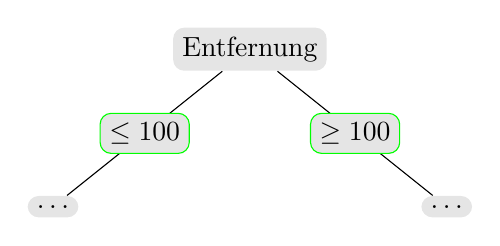
\begin{tikzpicture}
		[every node/.style={fill=black!10,rounded corners,align=center},
		grow=south, level distance=2cm,
		level 1/.style={sibling distance=5cm},
		level 2/.style={sibling distance=2cm},
		]

		\node{Entfernung}
			child{
				node{\(\dots\)} edge from parent node[draw=green]{\(\leq 100\)}}
			child{
				node{\(\dots\)} edge from parent node[draw=green]{\(\geq 100\)}}
		% es dürfen keine Leerzeilen dazwischen sein
			;
	\end{tikzpicture}
\end{figure}

Da \(H(Y|E \leq 100) = 0\), muss diese Datenmenge nicht weiter untereilt werden.
Jedoch ist \(H(Y|E > 100) > 0\).
Für die Daten, für die \(E \> 100\) gilt, wird das Verfahren rekursiv fortgeführt, bis alle Attribute verwendet sind oder der verbleibende Informationsgewinn 0 ist.
Es ergibt sich der Entscheidungsbaum aus Abbildung \ref{fig:EntscheidungsbaumBsp}.

Vorteile von Entscheidungsbäumen:
\begin{itemize}
	\item Kriterien des Entscheidungsbaums sind nachvollziehbar, keine Blackbox (Im Gegensatz zu neuronalen Netzen). 
	\item Wichtigkeit der Kriterien anhand der Position im Entscheidungsbaum erkennbar.
		Interessant für Marktforschung und verkleinern des Entscheidungsbaums, fals er schlecht generalisiert.
\end{itemize}
Nachteile von Entscheidungsbäumen:
\begin{itemize}
	\item Der Algorithmus kann nicht erkennen, ob ein Attribut mit hoher Entropie sinnvoll ist, z.B. Kreditkartennummer.
	\item Stetige Attribute müssen diskretisiert werden.
\end{itemize}

\subsubsection{Übung}
Gegeben sei nachfolgenden Trainigsdaten von Pilzen.
Erstellen Sie einen Entscheidungsbaum für das Attribut Essbar.
\begin{table}[htbp]
	\centering
	\begin{tabular}{cccc}
		\toprule
		\textbf{Farbe} & \textbf{Größe} & \textbf{Punkte} & \textbf{Essbar}	\\
		\midrule
		rot & klein & ja & nein\\
		braun & klein & nein & ja\\
		braun & groß & ja & ja\\
		grün & klein & nein & ja\\
		rot & groß & nein & ja	\\
		\bottomrule
	\end{tabular}
\end{table}

\begin{eqnarray*}
	H(Y)	&=& -(\frac{1}{5} \cdot \log_2(\frac{1}{5}) + \frac{4}{5} \cdot \log_2(\frac{4}{5}))	\\
			&=& 0,722\\\\
	G(Y,F)	&=& H(Y) - E H(Y|F)\\
			&=& 0,722 - (\frac{2}{5} \cdot 1 + \frac{2}{5} \cdot 0 + \frac{1}{5} \cdot 0)			\\
			&=& 0,322\\
	H(Y|F=\textrm{rot})		&=& \log_2 2 = 1\\
	H(Y|F=\textrm{braun})	&=& \log_2 1 = 0\\
	H(Y|F=\textrm{grün})	&=& \log_2 1 = 0
\end{eqnarray*}
\begin{eqnarray*}
	G(Y,G)	&=& H(Y) - E H(Y|G)\\
			&=& 0,722 - (\frac{3}{5} \cdot 0,918 + \frac{2}{5} \cdot 0)			\\
			&=& 0,171\\
	H(Y|G=\textrm{klein})	&=& -(\frac{2}{3} \cdot \log_2(\frac{2}{3}) + \frac{1}{3}\cdot \log_2(\frac{1}{3})) = 0,918\\	
	H(Y|G=\textrm{groß})	&=& \log_2 1 = 0	\\
	\\
	G(Y,P)	&=& H(Y) - E H(Y|P)\\
			&=& 0,722 - (\frac{2}{5} \cdot 1 + \frac{3}{5} \cdot 0)			\\
			&=& 0,322\\
	H(Y|P=\textrm{ja})	&=& \log_2 2 = 1\\
	H(Y|P=\textrm{nein})	&=& \log_2 1 = 0
\end{eqnarray*}
Das Attribut Punkte hat den größten Informationsgewinn und steht somit an oberster Stelle.
Es wird jetzt rekursiv die nächsten Ebenen berechnet
\begin{eqnarray*}
	H(Y|P=\textrm{nein})		&=& -(\frac{3}{3} \cdot \log_2 \frac{3}{3})	\\
								&=& 0
\end{eqnarray*}
Da die Entropie für das Attribut keine Punkte gleich 0 ist, muss dieses nicht weiter untereilt werden.
\begin{eqnarray*}
	H(Y|P=\textrm{ja})			&=& -(\frac{1}{2} \cdot \log_2 \frac{1}{2})	\\
								&=& 1	\\
	G(Y|F,P=\textrm{ja})		&=& H(Y) - E H(Y|F)\\
								&=& 1 - (\frac{1}{2} \cdot 0 + \frac{1}{2} \cdot 0)	\\
								&=& 1\\
	H(Y|F=\textrm{rot}, P=\textrm{ja})		&=& 1 \cdot \log_2 1 = 0\\
	H(Y|F=\textrm{braun}, P=\textrm{ja})	&=& 1 \cdot \log_2 1 = 0\\
	\\
	G(Y|G,P=\textrm{ja})		&=& H(Y) - E H(Y|F)\\
								&=& 1 - (\frac{1}{2} \cdot 0 + \frac{1}{2} \cdot 0)	\\
								&=& 1\\
	H(Y|G=\textrm{groß}, P=\textrm{ja})		&=& 1 \cdot \log_2 1 = 0\\
	H(Y|G=\textrm{klein}, P=\textrm{ja})	&=& 1 \cdot \log_2 1 = 0\\
\end{eqnarray*}
Da der Informationsgewinn für das Attribut Farbe und Größe gleich ist, ist die Auswahl egal.
Wir wählen als nächstes Attribut Punkte.
\begin{eqnarray*}
	H(Y|P=\textrm{ja}, G=\textrm{klein})	&=& -(\frac{1}{1} \cdot \log_2 \frac{1}{1})	\\
								&=& 0	\\
	H(Y|P=\textrm{ja}, G=\textrm{groß})		&=& -(\frac{1}{1} \cdot \log_2 \frac{1}{1})	\\
								&=& 0
\end{eqnarray*}
Da die Entropie für beide Ausprägungen 0 ist, endet hier die Rekursion.
Eine weitere Einteilung würde keinen Informationsgewinn bringen
\begin{figure}[htbp]
	\centering
	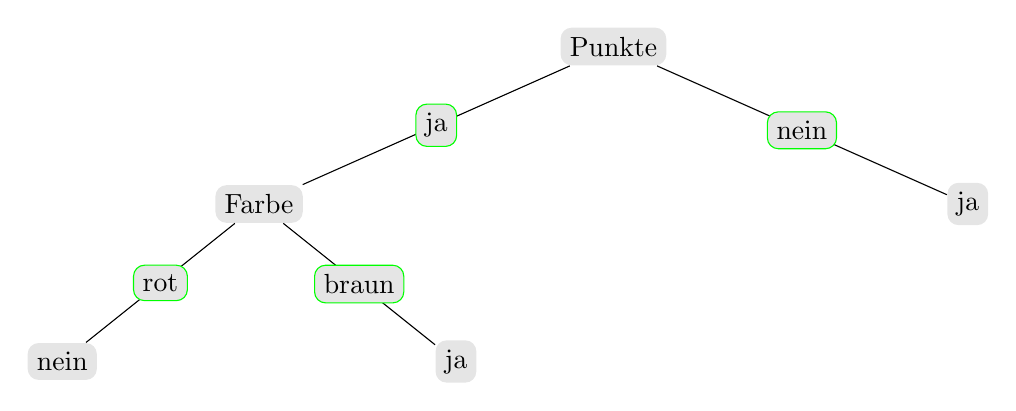
\begin{tikzpicture}
		[every node/.style={fill=black!10,rounded corners,align=center},
		grow=south, level distance=2cm,
		level 1/.style={sibling distance=9cm},
		level 2/.style={sibling distance=5cm},
		]

		\node{Punkte}
			child{
				node{Farbe}
					child{
						node {nein} edge from parent node[draw=green]{rot}}
					child{
						node {ja} edge from parent node[draw=green]{braun}}
					edge from parent node[draw=green]{ja}}
			child{
				node{ja} edge from parent node[draw=green]{nein}}
		% es dürfen keine Leerzeilen dazwischen sein
		;
	\end{tikzpicture}
	\caption{Entscheidungsbaum für die Klassifizierung ``Pilze essbar?''}
\end{figure}